\setlength{\columnsep}{3pt}
\begin{flushleft}

Starting with RHEL8, you can directly install package from Red Hat Network. 
\newline
For this, you need join a free Red Hat Developer program. 
\newline
Follow along for step-by-step guide:

\begin{itemize}
			\item Browse to \textbf{https://developers.redhat.com/register}.
			\item Create an account as shown in the image:
			\begin{figure}[h!]
				\centering
				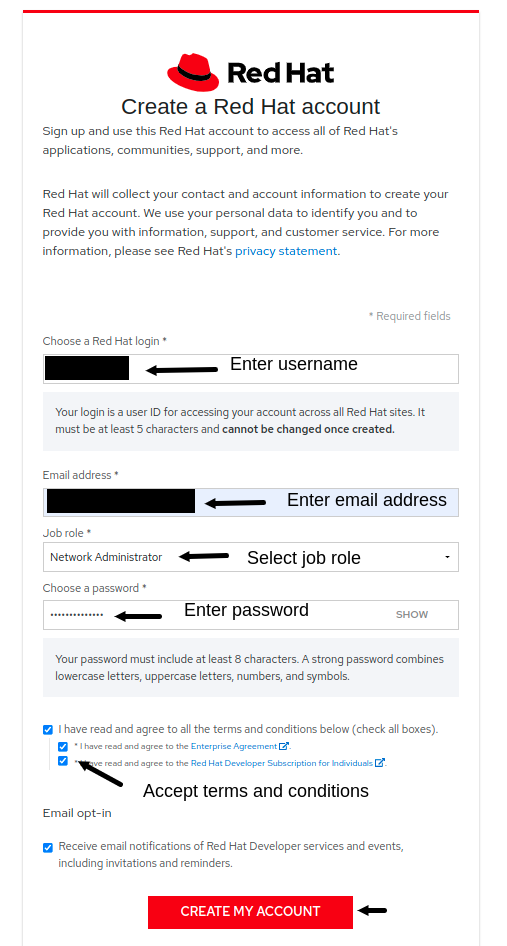
\includegraphics[scale=.4]{content/chapter11/images/account.png}
				\caption{Sample output}
				\label{fig:iso3}
			\end{figure}
		\newpage
			\item Once you have created your account, Red Hat should send a verification email as shown. Click on the link provided in email to confirm your email address.
			\begin{figure}[h!]
				\centering
				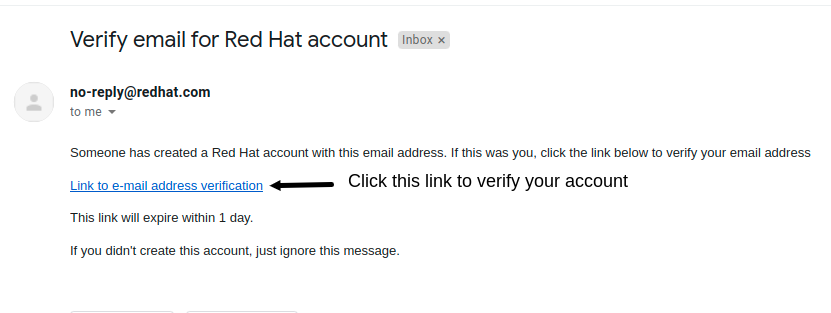
\includegraphics[scale=.25]{content/chapter11/images/verify.png}
				\caption{Sample output of verification email}
				\label{fig:iso4}
			\end{figure}
			\item Now register your RHEL8 server to Red Hat Network. Enter valid username and password that you created during account creation.
				\begin{tcolorbox}[breakable,notitle,boxrule=-0pt,colback=pink,colframe=pink]
				\color{black}
				\fontdimen2\font=9pt
				Syntax: subscription-manager register
				\fontdimen2\font=4pt
			\end{tcolorbox}
			Eg:
			\begin{figure}[h!]
				\centering
				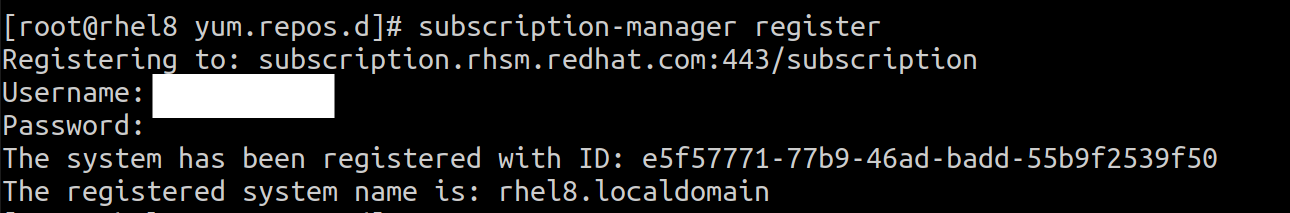
\includegraphics[scale=.2]{content/chapter11/images/2.png}
				\caption{Sample output}
				\label{fig:iso5}
			\end{figure}
			
			\bigskip
			\bigskip
			\item Confirm whether the system is successfully registered.
			\begin{tcolorbox}[breakable,notitle,boxrule=-0pt,colback=pink,colframe=pink]
				\color{black}
				\fontdimen2\font=9pt
				Syntax: subscription-manager status
				\fontdimen2\font=4pt
			\end{tcolorbox}
			Eg:
			\begin{figure}[h!]
				\centering
				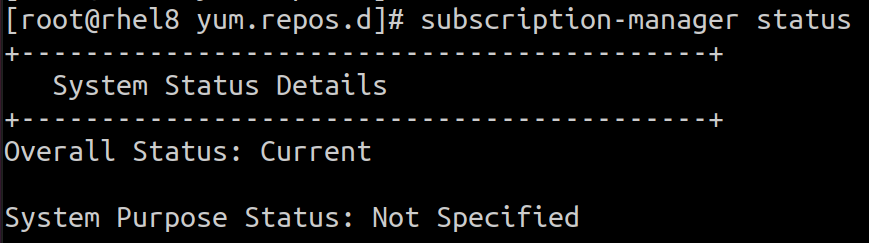
\includegraphics[scale=.3]{content/chapter11/images/3.png}
				\caption{Sample output}
				\label{fig:iso6}
			\end{figure}
			
			\newpage
			\item Finally, attach the subscriptions to your RHEL8 server.
			\begin{tcolorbox}[breakable,notitle,boxrule=-0pt,colback=pink,colframe=pink]
				\color{black}
				\fontdimen2\font=9pt
				Syntax: subscription-manager attach ---auto
				\fontdimen2\font=4pt
			\end{tcolorbox}
			Eg:
			\begin{figure}[h!]
				\centering
				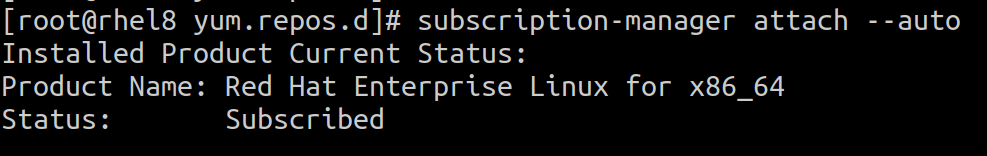
\includegraphics[scale=.3]{content/chapter11/images/4.png}
				\caption{Sample output}
				\label{fig:iso7}
			\end{figure}		
			\bigskip
						\bigskip
			\item Clear the yum cache.
			\begin{tcolorbox}[breakable,notitle,boxrule=-0pt,colback=pink,colframe=pink]
				\color{black}
				\fontdimen2\font=9pt
				Syntax: yum clean all
				\fontdimen2\font=4pt
			\end{tcolorbox}		
			\bigskip
						\bigskip
			\item Refresh yum repository.
			\begin{tcolorbox}[breakable,notitle,boxrule=-0pt,colback=pink,colframe=pink]
				\color{black}
				\fontdimen2\font=9pt
				Syntax: yum update all
				\fontdimen2\font=4pt
			\end{tcolorbox}		
			Eg:
			\begin{figure}[h!]
				\centering
				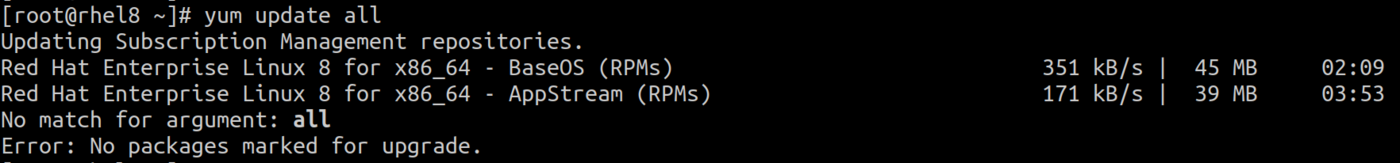
\includegraphics[scale=.25]{content/chapter11/images/update.png}
				\caption{Sample output}
				\label{fig:iso7}
			\end{figure}		
			\bigskip
			\bigskip
			\item Install httpd package to confirm you are connected to Red Hat Network.
			\bigskip
			\begin{tcolorbox}[breakable,notitle,boxrule=-0pt,colback=black,colframe=black]
				\color{white}
				\fontdimen2\font=9pt
				\color{green}
				\# yum install httpd -y
				\fontdimen2\font=4pt
			\end{tcolorbox}
\end{itemize}
	
		
		
	
	
\end{flushleft}

\newpage

